\documentclass{standalone}
\usepackage{tikz}
\begin{document}
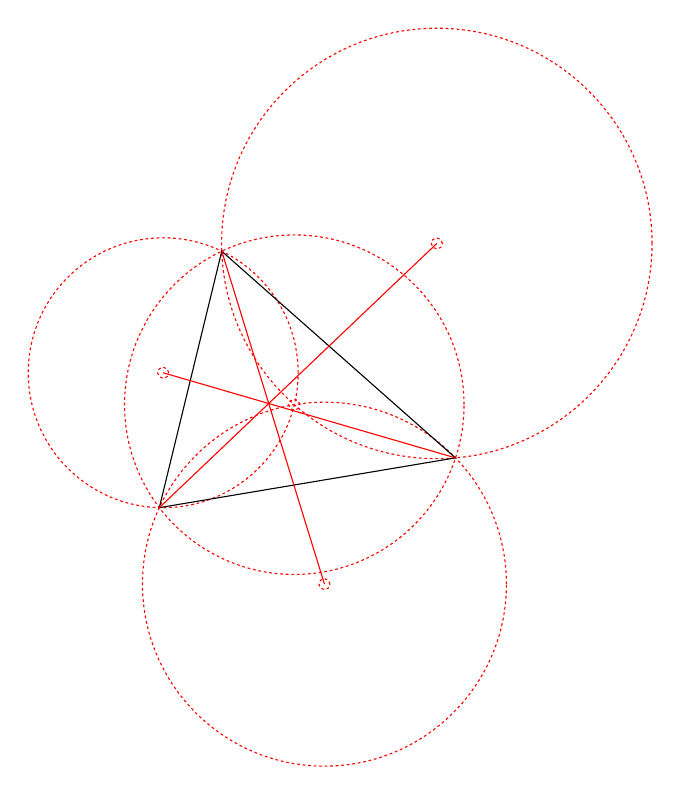
\begin{tikzpicture}[x=1pt,y=1pt]
\draw[red, dash pattern=on 1pt] (136.52,-154.65) circle (61.34);
\draw[red, dash pattern=on 1pt] (188.03,-96.39) circle (77.77);
\draw[red, dash pattern=on 1pt] (147.42,-219.50) circle (65.76);
\draw[red, dash pattern=on 1pt] (89.14,-143.12) circle (48.76);
\draw (110.31,-99.20) -- (87.75,-191.86) -- (194.77,-173.87) -- cycle;
\draw[red] (89.14,-143.12) -- (194.77,-173.87);
\draw[red] (188.03,-96.39) -- (87.75,-191.86);
\draw[red] (110.31,-99.20) -- (147.42,-219.50);
\draw[red, dash pattern=on 1pt] (136.52,-154.65) circle (2.00);
\draw[red, dash pattern=on 1pt] (89.14,-143.12) circle (2.00);
\draw[red, dash pattern=on 1pt] (188.03,-96.39) circle (2.00);
\draw[red, dash pattern=on 1pt] (147.42,-219.50) circle (2.00);
\end{tikzpicture}
\end{document}
